\documentclass[runningheads]{llncs}

\usepackage[T1]{fontenc}
\usepackage{graphicx}
% \renewcommand\UrlFont{\color{blue}\rmfamily}
\usepackage{hyperref}
\usepackage{color}
\usepackage{setspace}
\usepackage{verbatim}
\usepackage{multicol}
\usepackage{array}
\usepackage{bbding}
\usepackage{wasysym}

%----Making things more compact
\newcommand{\smalltt}[1]{\small \texttt{#1}}
\newenvironment{packed_itemize}{
\vspace*{-0.2em}
\begin{itemize}
\setlength{\partopsep}{0pt}
\setlength{\itemsep}{1pt}
\setlength{\parskip}{0pt}
\setlength{\parsep}{0pt}
}{\end{itemize}}
\newenvironment{packed_enumerate}{
\vspace*{-0.2em}
\begin{enumerate}
\setlength{\partopsep}{0pt}
\setlength{\itemsep}{1pt}
\setlength{\parskip}{0pt}
\setlength{\parsep}{0pt}
}{\end{enumerate}}
\renewcommand{\textfraction}{0.07}
\renewcommand{\topfraction}{0.9}
\renewcommand{\bottomfraction}{0.9}
\renewcommand{\floatpagefraction}{0.66}
% \setlength{\floatsep}{2.0pt plus 2.0pt minus 2.0pt}
% \setlength{\textfloatsep}{5.0pt plus 2.0pt minus 0.0pt}

\title{Automated Reasoning for Mathematics \\ in the TPTP World}

\author{
  Geoff Sutcliffe\orcidID{0000-0001-9120-3927}\Envelope
}

\institute{
  University of Miami,
  Miami, USA\\
  \email{geoff@cs.miami.edu}\\
}

\authorrunning{Geoff Sutcliffe}
\titlerunning{Mathematics in the TPTP World}

\begin{document}
\maketitle

%--------------------------------------------------------------------------------------------------
\begin{abstract}
The TPTP World is a well established infrastructure that supports research, development, and 
deployment of Automated Theorem Proving (ATP) systems.
A large portion of the TPTP is concerned with various mathematical domains.
This paper documents the mathematical domains of TPTP v9.0.0, and provides some insight into 
the performance of state-of-the-art ATP systems on the problems in these domains.
For those new to the field this information provides an established starting point for research.
For those already involved, this paper tells what has been achieved so far.
\end{abstract}
%--------------------------------------------------------------------------------------------------
\section{Introduction}
\label{Introduction}

Automated Reasoning is a subfield of artificial intelligence, dealing with computer systems
(largely software systems) that allow computers to reason completely, or nearly completely, 
automatically\footnote{%
Quoted from Wikipedia \href{https://en.wikipedia.org/wiki/Automated_reasoning}{{\tt en.wikipedia.org/wiki/Automated\_reasoning}}}~\cite{RV01-HAR}.
Automated reasoning spans a diversity of approaches, from deduction in logic~\cite{Gal15} to more 
forgiving types of reasoning such as argumentation~\cite{vE+14}.
The left side of Figure~\ref{UseOfAR} shows how automated reasoning systems are used in general: 
(i)~a world problem written in an application domain language is translated to the language
of the automated reasoning system; (ii)~the resultant reasoning problem is given to an automated 
reasoning system; (iii)~the automated reasoning system produces a solution (which can be in a
language different from that used for the problem); (iv)~the solution is translated to the 
application domain language.

For automated reasoning in mathematics, the mathematical problems are very often translated to 
a formal logic language, and the automated reasoning systems used to solve the problems are 
Automated Theorem Proving (ATP) systems~\cite{Bun83,RV01-HAR}.
The right side of Figure~\ref{UseOfAR} shows the specialization of general automated reasoning
to mathematical reasoning in logic:
(i)~a mathematical problem written in a mathematical language is translated to an appropriate 
logic language, as a set of axioms that model the mathematical domain and typically accompanied 
by a conjecture that formalizes a theorem to be proved; (ii)~the resultant logic problem is given 
to an ATP system; (iii)~the ATP system produces a solution in a logic language (which can be 
a different language from that used to write the problem); (iv)~the logic solution is translated 
to the mathematical language.

\begin{figure}[htb]
\centering
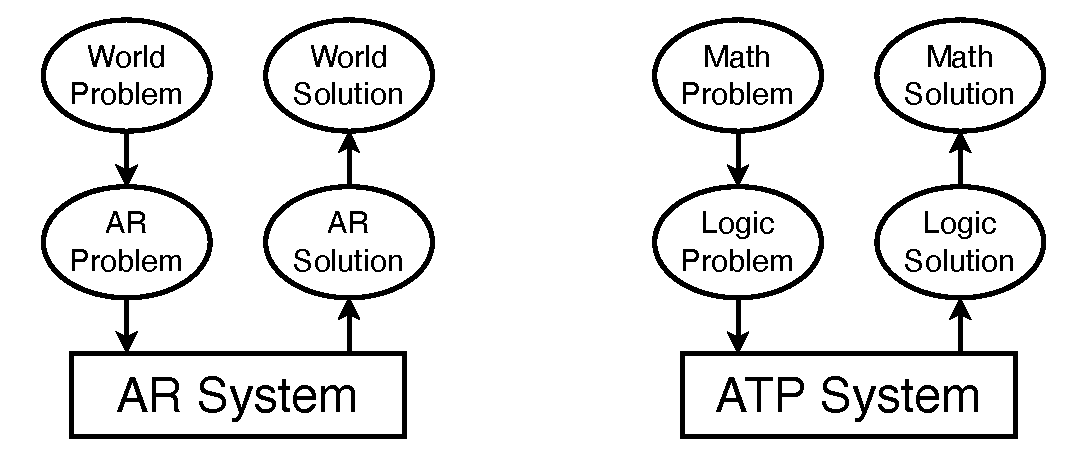
\includegraphics[width=0.6\textwidth]{UseOfAR.pdf}
\vspace*{-1em}
\caption{Use of Automated Reasoning}
\label{UseOfAR}
\end{figure}

The TPTP World is a well established infrastructure that supports research, development, and 
deployment of ATP~\cite{Sut10,Sut17}.
A large portion of the TPTP World is concerned with various mathematical domains.
This paper describes the data sets and services in the TPTP World that support automated reasoning
in mathematics.
Section~\ref{TPTPWorld} provides the necessary background about the TPTP World.
Section~\ref{MathProblems} describes the breadth and depth of mathematical problems in the TPTP
World.
Section~\ref{MathSolutions} covers the solutions to mathematical problems in the TPTP World,
including some details of outstanding results in mathematics achieved with ATP.
Section~\ref{Conclusion} concludes.

This section describes the parts of the TPTP World that are referred to in the subsequent sections 
that describe the mathematics in the TPTP World.
Salient components of the TPTP World are
the TPTP language that is used to write mathematical problems and solutions as logic problems and 
solutions (Section~\ref{Languages}),
the TPTP problem library and TSTP solution library that contain (amoung others) mathematical
problems and solutions (Sections~\ref{TPTP} and~\ref{TSTP}),
the problem and ATP systems ratings that indicate how hard (the mathematical) problems are and 
how strong the ATP systems are (Section~\ref{Ratings}),
and SystemOnTPTP for executing ATP systems and tools on the mathematical problems and solutions
(Section~\ref{SystemOnTPTP}).
The web page \href{http://www.tptp.org}{{\tt www.tptp.org}} provides access to all components.

%--------------------------------------------------------------------------------------------------
\section{The TPTP Language}
\label{Languages}

The TPTP language~\cite{Sut23-IGPL} is one of the keys to the success of the TPTP World.
The TPTP language is used for writing both problems and solutions,
which enables convenient communication between ATP systems and tools.
The TPTP language supports propositional, first-order, typed first-order, higher-order, and
non-classical logics, each of which is useful for different types of mathematics.

Problems and solutions are built from {\em annotated formulae} of the form: \\
\hspace*{0.5cm}{\em language}{\tt (}{\em name}{\tt ,}
{\em role}{\tt ,}
{\em formula}{\tt ,}
{\em source}{\tt ,}
{\em useful\_info}{\tt )}\\
The {\em language}s supported are {\smalltt{cnf}} (clause normal form), {\smalltt{fof}}
(first-order form), {\smalltt{tff}} (typed first-order form), and {\smalltt{thf}}
(typed higher-order form).
The {\em role}, e.g., {\smalltt{axiom}}, {\smalltt{lemma}}, {\smalltt{conjecture}}, defines the 
use of the formula.
In a {\em formula}, terms and atoms follow Prolog conventions -- functions and predicates start 
with a lowercase letter or are {\tt '}single quoted{\tt '}, and variables start with an uppercase 
letter.
The language also supports interpreted symbols that either start with a {\tt \$}, e.g., the 
truth constants {\smalltt{\$true}} and {\smalltt{\$false}}, or are composed of 
non-alphabetic characters, e.g., integer/rational/real numbers such as 27, 43/92, -99.66.
The logical connectives in the TPTP language are
{\tt !}, {\tt ?}, {\tt {\raisebox{0.4ex}{\texttildelow}}}, {\tt |}, {\tt \&}, {\tt =>}, {\tt <=},
{\tt <=>}, and {\tt <{\raisebox{0.4ex}{\texttildelow}}>},
for the mathematical connectives
$\forall$, $\exists$, $\neg$, $\vee$, $\wedge$, $\Rightarrow$, $\Leftarrow$, $\Leftrightarrow$, 
and $\oplus$ respectively.
Equality and inequality are expressed as the infix operators {\tt =} and {\tt !=}.
The {\em source} and {\em useful\_info} are optional.
Figures~\ref{ExampleFOF} and~\ref{ExampleTF0} in Section~\ref{TPTP} show examples of formulae in
problems, and Figure~\ref{ExampleDerivationFormulae} shows examples of formulae in a proof.

%--------------------------------------------------------------------------------------------------
\section{Mathematical Problems in the TPTP World}
\label{TPTP}

The TPTP problem library is a comprehensive library of test problems for ATP systems~\cite{Sut09}.
It supports necessary for meaningful ATP system evaluations, meaningful system comparisons, 
repeatability of testing, and the production of statistically significant results. 
Seven main fields are defined: logic, mathematics, computer science, science \& engineering, 
social sciences, arts \& humanities, and other. 
Each field is subdivided into domains based mainly on the Dewey Decimal Classification and the 
Mathematics Subject Classification, and each domain identified by a three-letter mnemonic.
For a given {\em abstract} (mathematical) problem, the TPTP problem library can have multiple 
concrete {\em versions}, which are the problems that ATP systems solve. 

\begin{table}[tb]
\begin{center}
\setlength{\tabcolsep}{4pt}
\begin{tabular}{lr|rr|rrrr}
Domain              & TLM       & Abs  & Ver  & Equ  & Thm  & Prv  & Rtg \\
\hline
Arithmetic          & {\tt ARI} &  681 &  693 &  367 &  668 &  663 & 0.11 \\
Set theory          & {\tt SET} & 2443 & 1429 & 1324 & 1118 & 1083 & 0.47 \\
Graph theory        & {\tt GRA} &  116 &  175 &   55 &  108 &   83 & 0.55 \\
Relation algebra    & {\tt REL} &   53 &  223 &  223 &  218 &  212 & 0.50 \\
MV algebras         & {\tt MVA} &   15 &   15 &   15 &   15 &    4 & 0.94 \\
Boolean algebra     & {\tt BOO} &  105 &  150 &  149 &   79 &   79 & 0.49 \\
Robbins algebra     & {\tt ROB} &   34 &   48 &   47 &   34 &   25 & 0.63 \\
Left distributive   & {\tt LDA} &   41 &   50 &   50 &   23 &    7 & 0.77 \\
Lattices            & {\tt LAT} &  401 &  758 &  746 &  628 &  531 & 0.69 \\
Quantales           & {\tt QUA} &   21 &   21 &   21 &   20 &    8 & 0.72 \\
Kleene algebra      & {\tt KLE} &  182 &  257 &  257 &  238 &  209 & 0.50 \\
Groups              & {\tt GRP} &  821 & 1207 & 1078 & 1045 &  965 & 0.35 \\
Rings               & {\tt RNG} &  128 &  268 &  259 &  226 &  215 & 0.47 \\
Fields              & {\tt FLD} &  101 &  281 &    0 &  187 &  169 & 0.56 \\
Linear algebra      & {\tt LIN} &   15 &   15 &   15 &   15 &    0 & -    \\
Homological algebra & {\tt HAL} &    7 &   10 &   10 &    6 &    6 & 0.33 \\
Real algebra        & {\tt RAL} &   70 &   70 &   70 &   70 &    0 & -    \\
General Algebra     & {\tt ALG} &  444 &  551 &  549 &  487 &  418 & 0.42 \\
Number Theory       & {\tt NUM} & 1008 & 1811 & 1525 & 1204 & 1006 & 0.55 \\
Topology            & {\tt TOP} &   53 &  136 &  110 &  112 &   76 & 0.67 \\
Analysis            & {\tt ANA} &  140 &  209 &  187 &  198 &  135 & 0.45 \\
Geometry            & {\tt GEO} &  659 &  982 &  716 &  853 &  678 & 0.45 \\
Category Theory     & {\tt CAT} &   38 &  136 &  135 &  103 &   88 & 0.51 \\
\hline
Total               &           & 7656 &11778 &10132 & 7655 & 6660 & 0.46 \\
\end{tabular}
\end{center}
\caption{TPTP mathematical domain problems}
\label{Domains}
\end{table}

Table~\ref{Domains} lists the mathematical domains in the TPTP problem library v9.0.0.
The data columns provide the number of abstract problems, the number of problem versions, the
number of problems with equality, the number of problems whose conjctures are known to be
theorems, the number of those theorms that have been proved by some ATP system, and the average 
difficulty rating (0.00 means easy, 1.00 means unsolved -- see Secion~\ref{Characteristics}) over 
all the problems.

ARI SET SEU SEV GRA REL MVA BOO ROB LDA LAT QUA KLE GRP RNG FLD LIN HAL RAL ALG NUM NUN TOP ANA GEO CAT

Each TPTP problem version problem is stored in a separate physical file, using the naming scheme 
{\em DDDNNNFV}.
{\em DDD} is the domain mnemonic, {\em NNN} is the index of the abstract problem in the domain,
{\em F} identifies the TPTP language, and {\em V} is the version index in the abstract problem.
Each TPTP problem file has three parts: a header, optional includes, and annotated formulae.
The header section contains information for users, as shown in Figure~\ref{ExampleHeader}.
The header fields are self-explanatory, but of particular interest are the {\tt Status}, SPC,
and Rating fields, which are explained in Section~\ref{Characteristics}.
The include section of a problem file is optional, and if used contains {\tt include} directives 
for axiom files, as in Figure~\ref{ExampleFOF}.
Inclusion avoids the need for duplication of the formulae in commonly used axiomatizations.
The TPTP World has many axiomatizations of mathematical theories.
Figure~\ref{ExampleFOF} shows the include section and annotated formulae of the group theory 
problem {\tt GRP194+1}, written in first-order logic, and Figure~\ref{ExampleTF0} shows a cutdown 
version of the set theory problem {\tt SEV421\_1}, written in typed first-order logic.\footnote{%
TPTP problems can be browsed at \href{https://tptp.org/TPTP/}{{\tt tptp.org/TPTP/}}}

\begin{figure}[htb]
\centering
{\scriptsize
{\setlength{\baselineskip}{2.5mm}
\begin{verbatim}
%------------------------------------------------------------------------------
% File     : GRP194+1 : TPTP v9.0.0. Released v2.0.0.
% Domain   : Group Theory (Semigroups)
% Problem  : In semigroups, a surjective homomorphism maps the zero
% Version  : [Gol93] axioms.
% English  : If (F,*) and (H,+) are two semigroups, phi is a surjective
%            homomorphism from F to H, and id is a left zero for F, then 
%            phi(id) is a left zero for H.

% Refs     : [Gol93] Goller (1993), Anwendung des Theorembeweisers SETHEO a
% Source   : [Gol93]
% Names    :

% Status   : Theorem
% Rating   : 0.18 v9.0.0, 0.22 v7.5.0, 0.36 v6.1.0, 0.47 v6.0.0, 0.50 v5.3.0
% Syntax   : Number of formulae    :    8 (   2 unt;   0 def)
%            Number of atoms       :   21 (   4 equ)
%            Maximal formula atoms :    4 (   2 avg)
%            Number of connectives :   13 (   0   ~;   0   |;   6   &)
%                                         (   1 <=>;   6  =>;   0  <=;   0 <~>)
%            Maximal formula depth :    8 (   5 avg)
%            Maximal term depth    :    3 (   1 avg)
%            Number of predicates  :    3 (   2 usr;   0 prp; 2-2 aty)
%            Number of functors    :    5 (   5 usr;   3 con; 0-3 aty)
%            Number of variables   :   15 (  14   !;   1   ?)
% SPC      : FOF_THM_RFO_SEQ

% Comments :
%------------------------------------------------------------------------------
\end{verbatim}
}}
\caption{Header of problem {\tt GRP194+1}}
\label{ExampleHeader}
\end{figure}

\begin{figure}[h!]
\centering
{\footnotesize
{\setlength{\baselineskip}{3mm}
\begin{verbatim}
%------------------------------------------------------------------------
%----Include semigroup axioms
include('Axioms/GRP007+0.ax').
%------------------------------------------------------------------------
%----Definition of a homomorphism
fof(homomorphism1,axiom,
    ! [X] :
      ( group_member(X,f) => group_member(phi(X),h) ) ).

fof(homomorphism2,axiom,
    ! [X,Y] :
      ( ( group_member(X,f) & group_member(Y,f) )
     => multiply(h,phi(X),phi(Y)) = phi(multiply(f,X,Y)) ) ).

fof(surjective,axiom,
    ! [X] :
      ( group_member(X,h)
     => ? [Y] : ( group_member(Y,f) & phi(Y) = X ) ) ).

%----Definition of left zero
fof(left_zero,axiom,
    ! [G,X] :
      ( left_zero(G,X)
    <=> ( group_member(X,G)
        & ! [Y] : ( group_member(Y,G) => multiply(G,X,Y) = X ) ) ) ).

fof(left_zero_for_f,hypothesis,
    left_zero(f,f_left_zero) ).

fof(prove_left_zero_h,conjecture,
    left_zero(h,phi(f_left_zero)) ).
%------------------------------------------------------------------------
\end{verbatim}
}}
\caption{Group theory problem {\tt GRP194+1} in first-order logic}
\label{ExampleFOF}
\end{figure}

\begin{figure}[htb]
\centering
{\footnotesize
{\setlength{\baselineskip}{3mm}
\begin{verbatim}
%------------------------------------------------------------------------
tff(set_type,type,          set:          $tType ).
tff(element_type,type,      element:      $tType ).

tff(empty_set_decl,type,    empty_set:    set ).
tff(member_decl,type,       member:       ( element * set ) > $o ).
tff(subset_decl,type,       subset:       ( set * set ) > $o ).
tff(intersection_decl,type, intersection: ( set * set ) > set ).
tff(union_decl,type,        union:        ( set * set ) > set ).
tff(cardinality_decl,type,  cardinality:  set > $int ).

tff(empty_set,axiom,
    ! [S: set] :
      ( ! [X: element] : ~ member(X,S) <=> ( S = empty_set ) ) ).

tff(subset,axiom,
    ! [A: set,B: set] :
      ( subset(A,B)
    <=> ! [X: element] : ( member(X,A) => member(X,B) ) ) ).

tff(intersection,axiom,
    ! [X: element,A: set,B: set] :
      ( member(X,intersection(A,B)) <=> ( member(X,A) & member(X,B) )) ).

tff(union,axiom,
    ! [X: element,A: set,B: set] :
      ( member(X,union(A,B)) <=> ( member(X,A) | member(X,B) ) ) ).

tff(cardinality_empty_set,axiom,
    ! [S: set] :
      ( ( cardinality(S) = 0 ) <=> ( S = empty_set ) ) ).

tff(about_empty_sets,conjecture,
    ! [X: element,C: set,Size: $int] :
      ( ( ~ member(X,C) & ( Size = cardinality(C) ) )
     => ( ( Size = 0 ) <=> ( C = empty_set ) ) ) ).
%------------------------------------------------------------------------
\end{verbatim}
}}
\caption{Set theory with arithemtic problem {\tt SEV421\_1} in typed first-order logic}
\label{ExampleTF0}
\end{figure}

AXIOMATIZATIONS HERE

%--------------------------------------------------------------------------------------------------
\subsection{Status, SPC, and Rating}
\label{Characteristics}

The ``Status'' of a TPTP problem, as in Figure~\ref{ExampleHeader}, is given as an SZS ontology 
value~\cite{Sut08-KEAPPA}
The ontologies~\cite{SZS03}) provide values to specify the logical status of problems and
solutions, and to describe logical data.
The Success ontology provides values for the logical status of a conjecture with respect to a 
set of axioms, e.g., a TPTP problem whose conjecture is a logical consequence of the axioms 
is tagged as a {\tt Theorem}.
The NoSuccess and Dataform ontologies are used in the output from ATP systems, as described in
Section~\ref{TSTP}.
The NoSuccess ontology provides reasons why an ATP system/tool has failed, e.g., an ATP system 
might report {\tt Timeout}, and the Dataform ontology provides values for describing logical 
data.
Some commonly used ontology values are listed in Figure~\ref{SZSTable}.

% \begin{figure}[htb]
% \centering
% 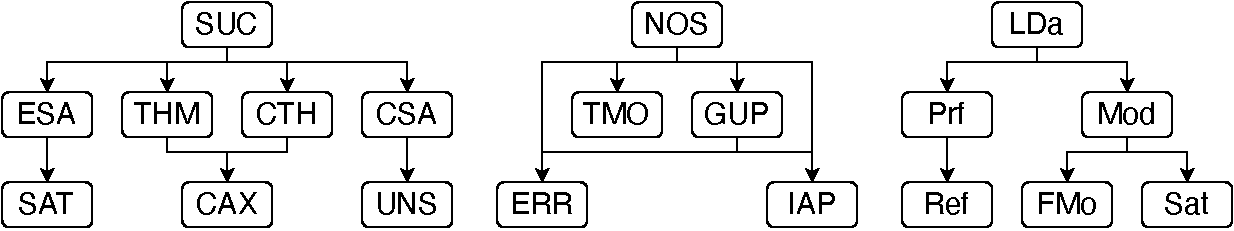
\includegraphics[width=0.75\textwidth]{SZSExtract.pdf}
% \caption{Extract of the SZS ontologies}
% \label{SZSExtract}
% \end{figure} 

\begin{figure}[htb]
\centering
\begin{tabular}{lll}
{\tt SZS} & Name                      & Meaning \\
\hline
{\tt THM} & {\tt Theorem}             & The conjecture is a theorem of the axioms \\
{\tt CAX} & {\tt ContradictoryAxioms} & The axioms are contradictory \\
{\tt SAT} & {\tt Satisfiable}         & The axioms are not contradictory \\
{\tt CSA} & {\tt CounterSatisfiable}  & The conjecture is not a theorem of the axioms \\
{\tt TMO} & {\tt Timeout}             & The ATP system stopped because of a time limit \\
{\tt GUP} & {\tt GaveUp}              & The ATP system gave up of its own accord \\
{\tt Prf} & {\tt Proof}               & The ATP system output is a proof \\
{\tt Mod} & {\tt Model}               & The ATP system output is a model \\
\end{tabular}
\caption{SZS ontology values}
\label{SZSTable}
\end{figure} 

The TPTP problem library is divided into Specialist Problem Classes (SPCs) of problems with 
recognizable logical, language, and syntactic characteristics, which make the problems in each 
SPC homogeneous wrt ATP systems.
An ATP system can be selected based on the SPC of the problem.
The characteristics used to define the SPC of a problem are the TPTP language variant, the SZS
status, the language order, use of equality, use of arithmetic.
The header shown in Figure~\ref{ExampleHeader} shows that {\tt GRP194+1} is in the 
SPC {\tt FOF\_THM\_RFO\_SEQ}, i.e., it's a first-order ({\tt FOF}) theorem ({\tt THM}) that
is really first-order ({\tt RFO} - cannot be reduced to propositional logic), and contains some
equality ({\tt SEQ}).
For anoth example, the SPC {\tt TF0\_THM\_NEQ\_ARI} contains typed monomorphic first-order theorems 
that have no equality but include arithmetic.

Each TPTP problem has a difficulty rating that provides a well-defined measure of how difficult 
the problem is for current ATP systems~\cite{SS01}.
The ratings are based on performance data in the TSTP solution library (see Section~\ref{TSTP}), 
done separately for each SPC.
The header shown in Figure~\ref{ExampleHeader} shows that {\tt GRP194+1} has a rating of 0.18 in
TPTP version v9.0.0, and had higher ratings in earlier TPTP releases.
Changes in difficulty ratings provide a way to assess progress in the field -- as problems that 
are unchanged are not actually getting easier, decreases in their difficulty ratings are evidence 
of progress in ATP systems.

%--------------------------------------------------------------------------------------------------
\section{Mathematical Solutions in the TPTP World}
\label{TSTP}

The complement to the TPTP problem library is the TSTP solution library~\cite{Sut07-CSR,Sut10}.
The TSTP is built by running all the ATP systems that are available in the TPTP World on
all the problems in the TPTP problem library.

Table~\ref{Proofs} lists BLAH BLAH.

\begin{table}[htb]
\begin{center}
\setlength{\tabcolsep}{4pt}
\begin{tabular}{lr|rrrrr}
Domain              & TLM       & Thm  & Prv  & Sys & Size & Depth \\
\hline
Arithmetic          & {\tt ARI} &  668 &  663 &     &      &       \\
Set theory          & {\tt SET} & 1118 & 1083 &     &      &       \\
Graph theory        & {\tt GRA} &  108 &   83 &     &      &       \\
Relation algebra    & {\tt REL} &  218 &  212 &     &      &       \\
MV algebras         & {\tt MVA} &   15 &    4 &     &      &       \\
Boolean algebra     & {\tt BOO} &   79 &   79 &     &      &       \\
Robbins algebra     & {\tt ROB} &   34 &   25 &     &      &       \\
Left distributive   & {\tt LDA} &   23 &    7 &     &      &       \\
Lattices            & {\tt LAT} &  628 &  531 &     &      &       \\
Quantales           & {\tt QUA} &   20 &    8 &     &      &       \\
Kleene algebra      & {\tt KLE} &  238 &  209 &     &      &       \\
Groups              & {\tt GRP} & 1045 &  965 &     &      &       \\
Rings               & {\tt RNG} &  226 &  215 &     &      &       \\
Fields              & {\tt FLD} &  187 &  169 &     &      &       \\
Linear algebra      & {\tt LIN} &   15 &    0 &     &      &       \\
Homological algebra & {\tt HAL} &    6 &    6 &     &      &       \\
Real algebra        & {\tt RAL} &   70 &    0 &     &      &       \\
General Algebra     & {\tt ALG} &  487 &  418 &     &      &       \\
Number Theory       & {\tt NUM} & 1204 & 1006 &     &      &       \\
Topology            & {\tt TOP} &  112 &   76 &     &      &       \\
Analysis            & {\tt ANA} &  198 &  135 &     &      &       \\
Geometry            & {\tt GEO} &  853 &  678 &     &      &       \\
Category Theory     & {\tt CAT} &  103 &   88 &     &      &       \\
\hline
Total               &           & 7656 &11778 &     &      &       \\
\end{tabular}
\end{center}
\caption{TPTP mathematical domain proofs}
\label{Proofs}
\end{table}

TSTP solution files have a header section and annotated formulae.
The header section has four parts, as shown in Figure~\ref{ExampleDerivationHeader}.
the first part identifies the ATP system, the problem, and the system's runtime parameters,
the second part provides information about the hardware, operating system, and resource limits,
the third part provides the SZS result and output values (see Section~\ref{Characteristics}), 
and syntactic characteristics of the solution; the last part contains comments.
The solution follows in annotated formulae.

\begin{figure}[htb]
\centering
{\scriptsize
{\setlength{\baselineskip}{2.5mm}
\begin{verbatim}
%------------------------------------------------------------------------------
% File     : E---3.2.5
% Problem  : GRP194+1 : TPTP v9.0.0. Released v2.0.0.
% Transfm  : none
% Format   : tptp:raw
% Command  : run_E %s %d THM

% Computer : n007.cluster.edu
% Model    : x86_64 x86_64
% CPU      : Intel(R) Xeon(R) CPU E5-2620 v4 2.10GHz
% Memory   : 8042.1875MB
% OS       : Linux 3.10.0-693.el7.x86_64
% CPULimit : 300s
% WCLimit  : 300s
% DateTime : Wed Apr  9 06:30:15 PM UTC 2025

% Result   : Theorem 0.21s 0.50s
% Output   : CNFRefutation 0.21s
% Verified : 
% SZS Type : Refutation
%            Derivation depth      :    7
%            Number of leaves      :    7
% Syntax   : Number of formulae    :   34 (  10 unt;   0 def)
%            Number of atoms       :   83 (  14 equ)
%            Maximal formula atoms :   11 (   2 avg)
%            Number of connectives :   86 (  37   ~;  35   |;   8   &)
%                                         (   1 <=>;   5  =>;   0  <=;   0 <~>)
%            Maximal formula depth :   12 (   4 avg)
%            Maximal term depth    :    4 (   1 avg)
%            Number of predicates  :    4 (   2 usr;   1 prp; 0-2 aty)
%            Number of functors    :    7 (   7 usr;   3 con; 0-3 aty)
%            Number of variables   :   47 (   1 sgn  22   !;   1   ?)

% Comments : 
%------------------------------------------------------------------------------
\end{verbatim}
}}
\caption{Header of a proof for {\tt GRP194+1}}
\label{ExampleDerivationHeader}
\end{figure}

For derivations, where formulae are derived from parent formulae, e.g., in proofs, refutations, 
etc., the {\em source} fields of the annotated formulae are used to capture parent-derived 
formulae relationships in the derivation DAG.
This includes the source of the formula -- either the problem file or an inference.
Inference data includes the name of the inference rule used, the semantic relationship between 
the parents and the derived formula as an SZS value, and a list of the parent annotated formulae 
names.
Figure~\ref{ExampleDerivationFormulae} shows an example refutation (slightly modified) from 
the E ATP system~\cite{SCV19} for the problem in Figure~\ref{ExampleFOF}, and 
Figure~\ref{ExampleDerivationHeader} shows the corresponding header.\footnote{%
TSTP solutions can be browsed at \href{https://tptp.org/TSTP/}{{\tt tptp.org/TSTP/}}}

\begin{figure}[h!]
\centering
{\footnotesize
{\setlength{\baselineskip}{3mm}
\begin{verbatim}
%------------------------------------------------------------------------
fof(total_function,axiom,
    ! [X1,X2,X3] :
      ( ( group_member(X2,X1) & group_member(X3,X1) )
     => group_member(multiply(X1,X2,X3),X1) ),
    file('Axioms/GRP007+0.ax',total_function) ).

fof(homomorphism2,axiom,
    ! [X2,X3] :
      ( ( group_member(X2,f) & group_member(X3,f) )
     => multiply(h,phi(X2),phi(X3)) = phi(multiply(f,X2,X3)) ),
    file('GRP194+1.p',homomorphism2) ).

... many proof steps here ...

fof(c_0_11,plain,
    ! [X14] :
      ( ( group_member(esk2_1(X14),f) | ~ group_member(X14,h) )
      & ( phi(esk2_1(X14)) = X14 | ~ group_member(X14,h) ) ),
    inference(distribute,[status(thm)],
      [inference(skolemize,[status(esa)],[surjective])]) ).

... many proof steps here ...

cnf(c_0_30,negated_conjecture,
    ~ left_zero(h,phi(f_left_zero)),
    inference(split_conjunct,[status(thm)],[c_0_26]) ).

cnf(c_0_31,hypothesis,
    ~ group_member(esk1_2(h,phi(f_left_zero)),h),
    inference(sr,[status(thm)],
      [inference(cn,[status(thm)],[inference(rw,[status(thm)],
        [inference(spm,[status(thm)],[c_0_27,c_0_28]),c_0_29])]),
      c_0_30]) ).

cnf(c_0_32,plain,
    ( group_member(esk1_2(X1,X2),X1)
    | left_zero(X1,X2) | ~ group_member(X2,X1) ),
    inference(split_conjunct,[status(thm)],[c_0_10]) ).

cnf(c_0_33,hypothesis,
    $false,
    inference(sr,[status(thm)],
      [inference(cn,[status(thm)],[inference(rw,[status(thm)],
        [inference(spm,[status(thm)],[c_0_31,c_0_32]),c_0_29])]),
      c_0_30]),
    [proof] ).
%------------------------------------------------------------------------
\end{verbatim}
}}
\caption{Extract from proof for {\tt GRP194+1}}
\label{ExampleDerivationFormulae}
\end{figure}

\begin{itemize}
\item Model finding ATP systems were used to solve previously open problems concerning the
      existence of quasigroups satisfying certain additional conditions \cite{SFS95}.
      Many examples are in the {\tt GRP} domain of the TPTP.
\item The solution of the Robbins problem\footnote{%
      The Robbins problem was posed in personal communications between Edward Huntington,
      Herbert Robbins, and Alfred Tarski.
      The background is given in
      \href{https://en.wikipedia.org/wiki/Robbins_algebra}{en.wikipedia.org/wiki/Robbins\_algebra}.}
      by the specialist ATP system EQP \cite{McC97}
      in 1996 was a noteworthy success, as the problem had defied the efforts of eminent
      mathematicians \cite{HMT71}.
      It is {\tt ROB001-1} in the TPTP, and still has a rating of 1.00 because
      it has not been solved by a non-specialist ATP system.
\item The first inner five-segment theorem of Tarski's geometry \cite{SST83} was first
      automatically proved by E \cite{Sch13-LPAR} in 2019, after being posed by Quaife in
      1989 \cite{Qua89}.
      It is problem {\tt GEO033-2} in the TPTP.
\item Larry Wos' challenge to find a ``circle of pure proofs'' that shows the equivalence
      of the four Moufang identities \cite{Wos19} was met by careful application \cite{Ver22} of
      Otter \cite{McC03-Otter} in 2021.
      While those specific problems are not in the TPTP, many related problems are in the
      ring theory ({\tt RNG}) domain of the TPTP.
\end{itemize}

%--------------------------------------------------------------------------------------------------
\section{Tools for Mathematicians}
\label{Tools}

The TPTP World understand that mathematicians are primarily concerned with mathematics, and would
use ATP as a convenient tool to support theor research.
With that in mind the TPTP World provide a suite of online services to make it easy to use ATP
systems and related tools.
While many users enjoy interactive use of the services in a web browser, it is also easy to use 
the services programmatically.
The core service is SystemOnTPTP~\cite{Sut00-CADE-17}, which provides hardware and interfaces 
for users to submit their problems to most recent versions of a wide range of ATP 
systems.\footnote{%
Available at \href{https://tptp.org/cgi-bin/SystemOnTPTP}{{\tt tptp.org/cgi-bin/SystemOnTPTP}}}
SystemOnTPTP can provide recommendations for ATP systems that might be most likely to solve
a problem, based on the SPC of the user's problem and the system ratings for the SPC
(see Section~\ref{Characteristics}).
SystemOnTPTP can also run ATP systems (e.g., the recommended systems) in competition
parallel~\cite{SS99-FLAIRS}.
The core SystemOnTPTP service is supported by (i)~the SystemB4TPTP service that provides tools to
prepare problems for submission to ATP systems,\footnote{%
Available at \href{https://tptp.org/cgi-bin/SystemB4TPTP}{{\tt tptp.org/cgi-bin/SystemB4TPTP}}}
e.g., axiom selection~\cite{HV11}, type 
checking~\cite{KSR16}, a scripting language~\cite{Sut14}, and (ii)~the SystemOnTSTP service that 
provides tools for analysing solutions,\footnote{%
Available at \href{https://tptp.org/cgi-bin/SystemOnTSTP}{{\tt tptp.org/cgi-bin/SystemOnTSTP}}} 
e.g., interactive viewing of derivations~\cite{TPS07}, proof checking~\cite{Sut06}, identification 
of interesting lemmas in a proof~\cite{PGS06}.

The Interactive Derivation Viewer (IDV) in SystemOnTSTP is of particular interest to mathematicians.
Figure~\ref{IDV} shows two views of the proof for {\tt GRP194+1} listed in 
Figure~\ref{ExampleDerivationFormulae}.
The lefthand side shows all the steps of the derivation.
The ``house'' in the top row is the conjecture, and the inverted triangles in the top row are the
axioms.
The inverted house is the negated conjecture, the ovals are steps in the proof, and the box at the
bottom is the {\tt \$false} node that completes the proof by refutation.
The lefthand panel shows the logical formulae when the mouse selects a node.
Many mathematical proofs have very many nodes, too many for easy consumption in the proof viewer.
IDV can help with its ability to measure the interestingness of each inferred formula, scale the
nodes according to their interestingness, and hide less interesting nodes.
This is shown in the righthand of Figure~\ref{IDV}.
For example, the largest node is {\tt c\_0\_29} which says that {\tt phi(f\_left\_zero)} is a 
member of the group {\tt h} (see Figure~\ref{ExampleFOF}).

\begin{figure}[htb]
\centering
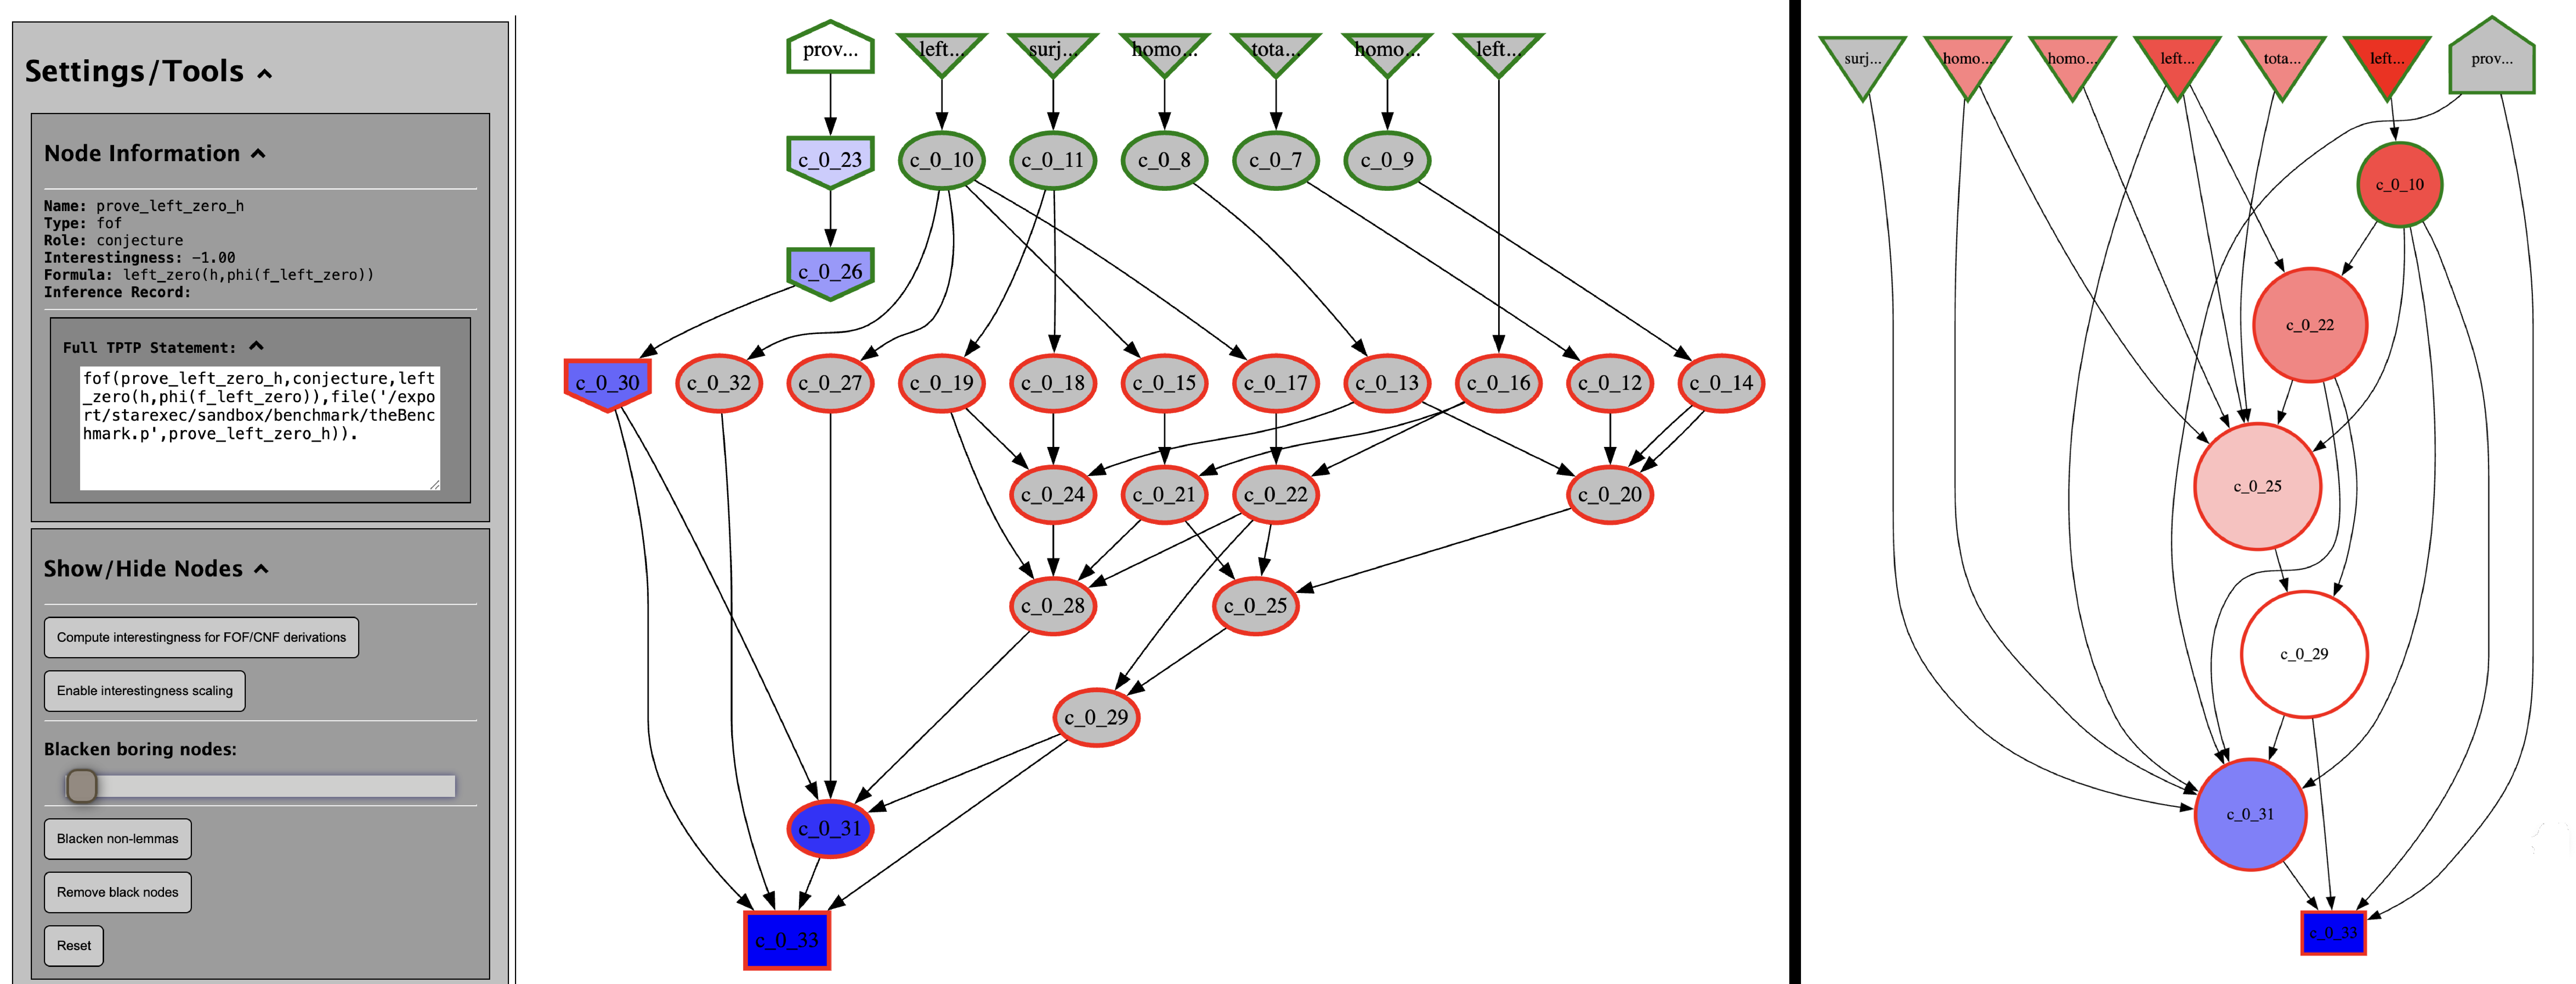
\includegraphics[width=1.0\textwidth]{IDV.pdf}
\vspace*{-1em}
\caption{IDV views of a proof for {\tt GRP194+1}}
\label{IDV}
\end{figure}

%--------------------------------------------------------------------------------------------------
\section{Conclusion}
\label{Conclusion}

This paper has described key components of the TPTP World that help make it a success,
linking them together as ``stepping stones'' that lead from one component to another.
The large number of citations to work of others, and explicitly Section~\ref{Users}, 
illustrate how the TPTP World has benefited, and benefited from, users in the ATP community.
I am also grateful to the many people who have donated hard cash to the project, helping
to keep it alive!

This paper has naturally focused on the successful parts of the TPTP World.
There have also been some failed developments and suboptimal (in retrospect) decisions \frownie{}.
For example, in 2015 there was an attempt to develop a description logic form for the TPTP 
language. 
While some initial progress was made, it ground to a halt without support from the description 
logic community.
A suboptimal design decision, rooted in the early days of the TPTP, is the naming scheme used for 
problem files. 
The naming scheme uses three digits to number the problems in each domain, thus setting a limit 
of 1000 problems, which failed to anticipate the numbers of problems that would be contributed 
to some of the problem domains.
This has been overcome by creating multiple domain directories where necessary, but if it were 
to be done again, six or eight digit problem numbers shared across all domains would be an 
improvement.

The maintenance and development of the TPTP World is ongoing work.
The most recent development is the languages and support for non-classical logics, initially
modal logic~\cite{SF+22,SS24}.
The new format for representing interpretations (see Section~\ref{TSTP}) will be promulgated in 
the near future.
As always, the ongoing success and utility of the TPTP problem library depends on ongoing 
contributions of problems -- the automated reasoning community is encouraged to continue making 
contributions of all types of problems.

The TPTP World would not exist without the early strategic insights of Christian Suttner,
with his willingness to let me do the organization without interference. 
Maybe his most wonderful contribution (which took him over two hours to produce when he
was visiting me at James Cook University -- I think he took a nap \smiley) is his 
wonderfully simple plain-language definition of automated theorem proving: 
``the derivation of conclusions that follow inevitably from known facts''.

%--------------------------------------------------------------------------------------------------
\bibliographystyle{splncs04}
\bibliography{Bibliography.bib}
%--------------------------------------------------------------------------------------------------
\end{document}
%--------------------------------------------------------------------------------------------------
